\label{Algorithm}
\section{Algorithm}

The algorithm we are presenting works on two main steps:
\begin{itemize}
  \item Build the data structure - the efficiency of the algorithm is determined by the data structure it runs on. On the other hand, the data structure is specifically designed to solve this problem.
  \item Traverse data structure and output result - the algorithm works by  discarding part of the information on every iteration, thereby reducing the size of the problem.
\end{itemize} 

\subsection{Notations}
Let G = (V,E) be an weighted, undirected simple graph and let n = \(\lvert V\rvert\) and m = \(\lvert E\rvert\).

A vertex v denotes an actor. Any edge e between vertices \(v_1\) and \(v_2\) denotes a set of movies these two actors have played together. Weight of the edge, W(e) denotes the size of that set.

Denote by A(v) the set of adjacent edges to vertex v.

SET(e) is the set of (two) vertices adjacent to an edge e.

Unique(\(v_1, v_2,... v_n)\) - returns a set of unique elements.

Remove(v) - removes edges adjacent to v from the graph G.

MovieCount denotes the biggest number found so far of common movies between any given three actors.

\subsection{Data structure}
As mentioned in the previous section, the algorithm works starts by first building the data structure. The data structure is a graph, where vertices represent actors and edges between them represent the movie(s) these actors played together in. 

\begin{figure}[ht!]
\centering
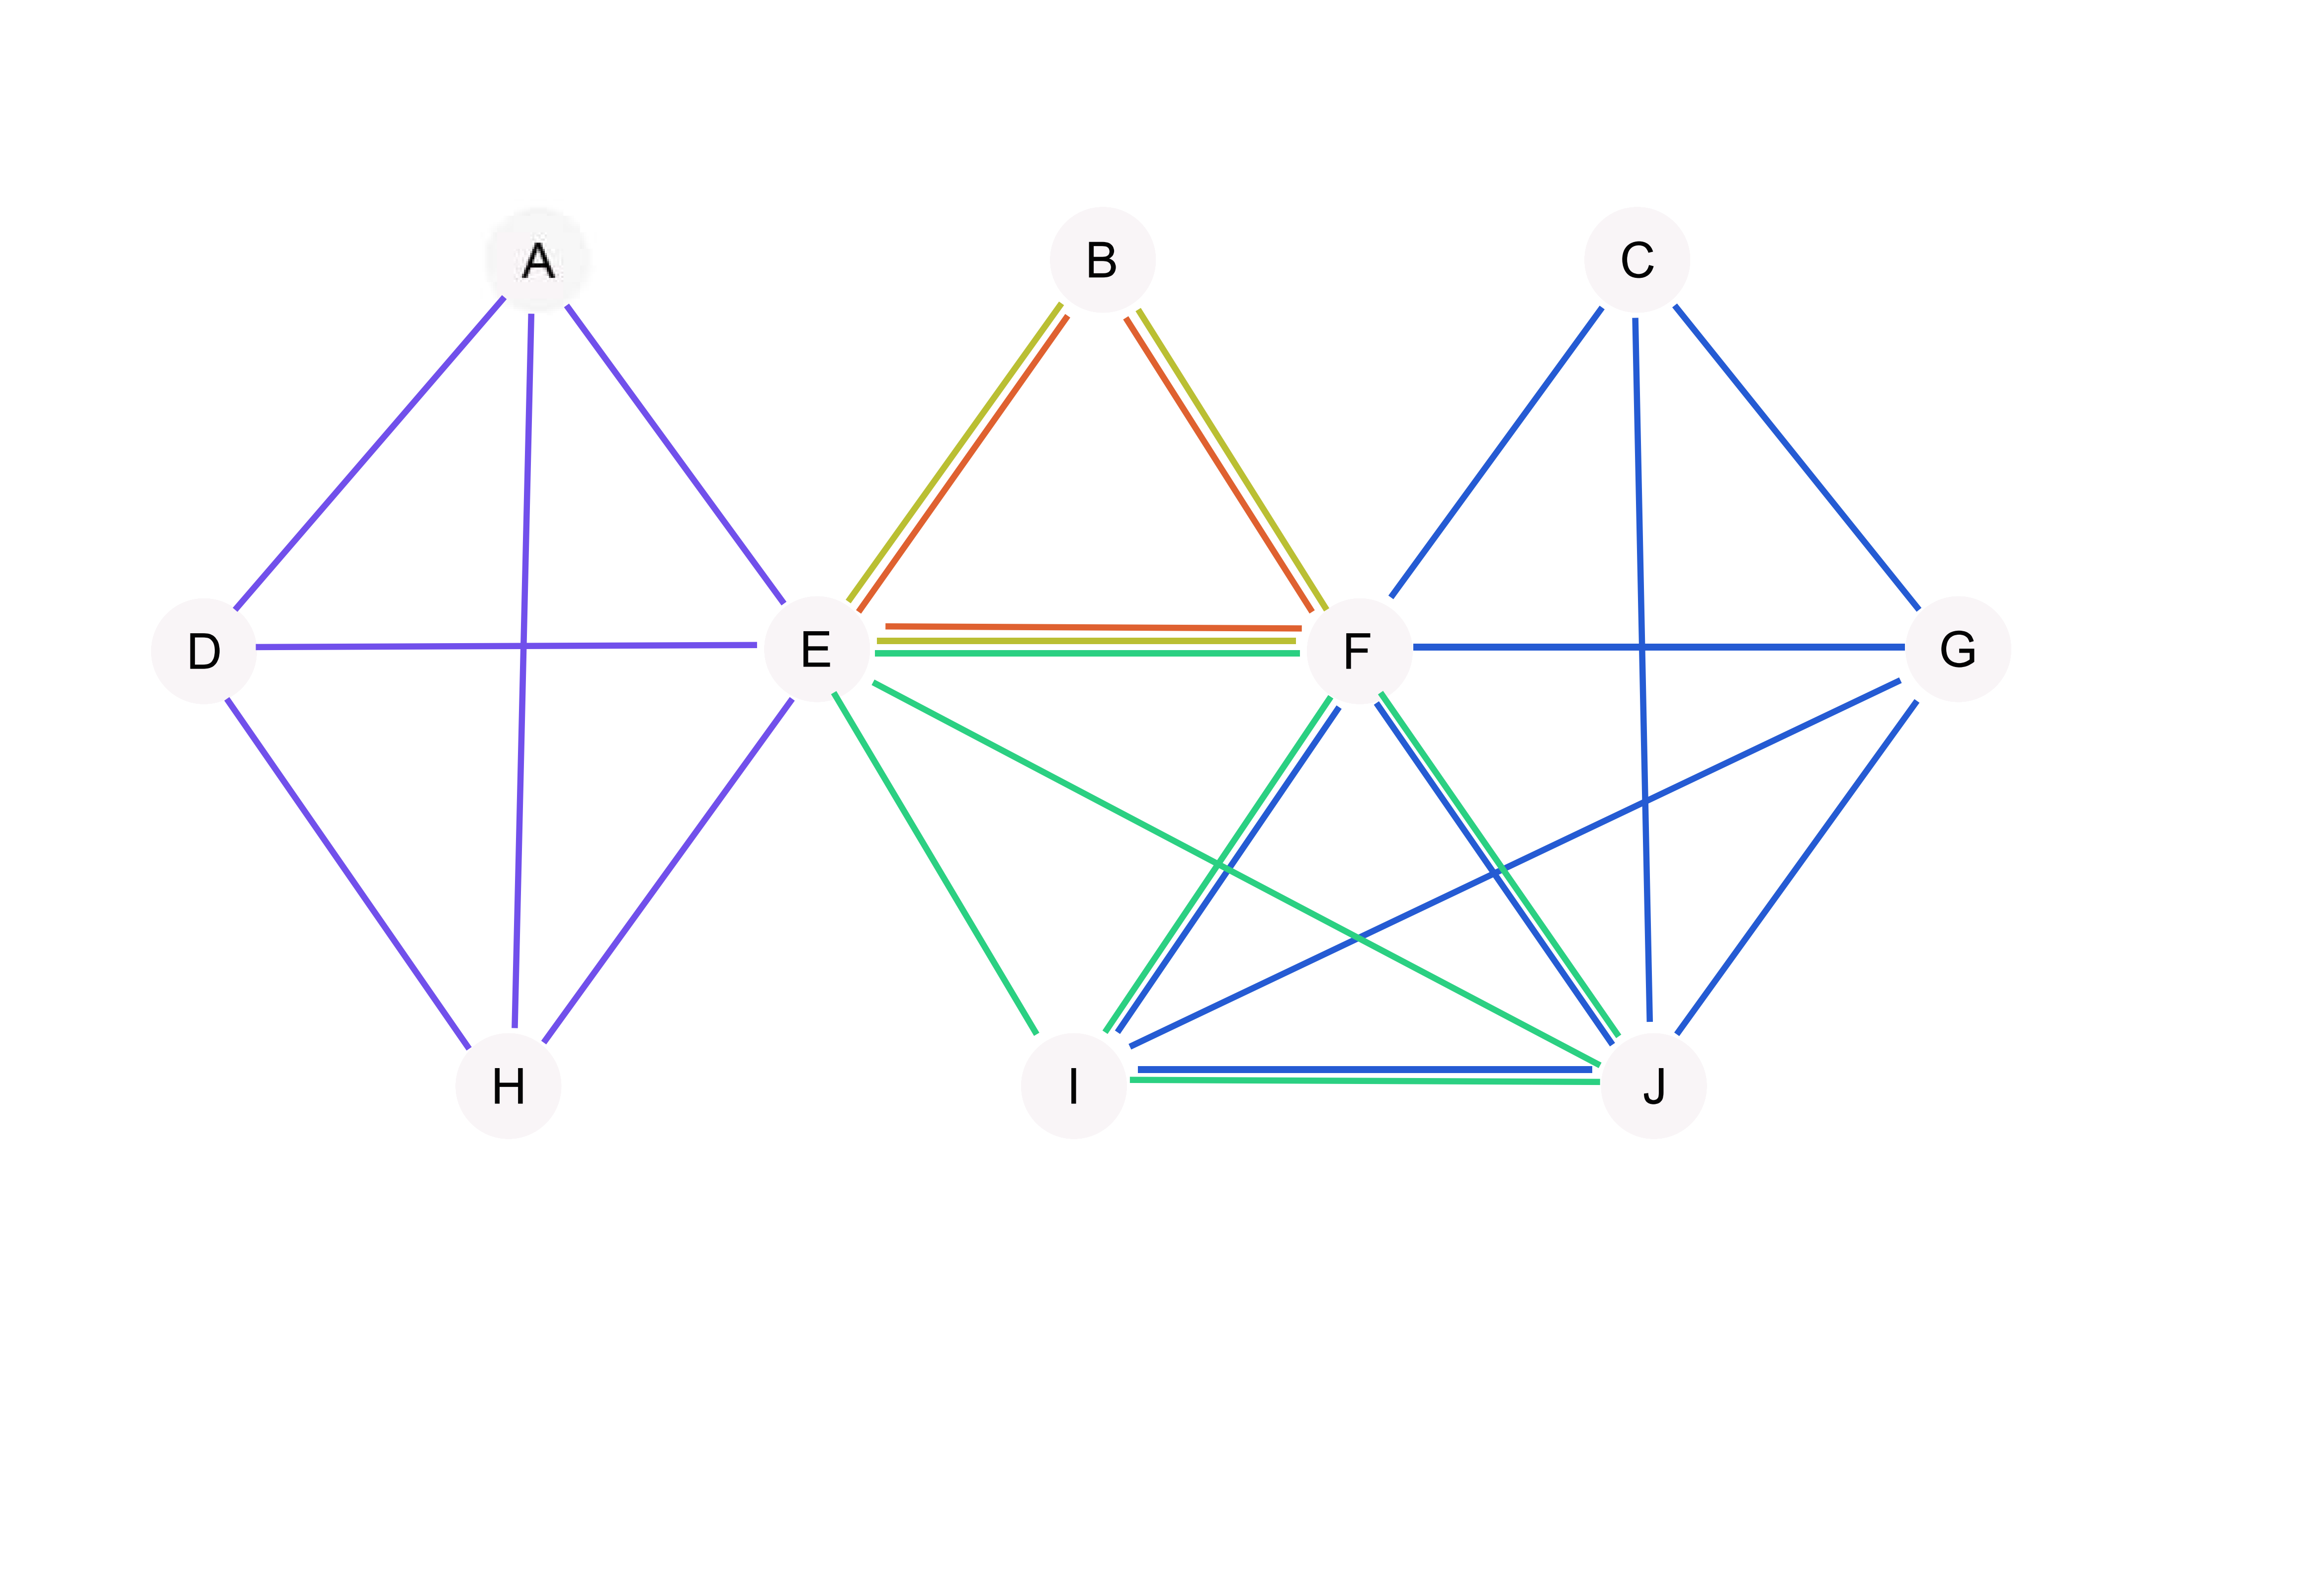
\includegraphics[width=130mm]{resources/project_problem_illustration.png}
\caption{Graph Example}
\label{example}
\end{figure}

Figure \ref{example} represents the data structure. To clearly illustrate the problem, the picture above represents a multi-graph, i.e. there can be multiple edges between two vertices. This is not the case of the actual data structure, however, as multiple edges are collapsed into a single one, where the weight is the sum of the weights of the original edges. The weight of an edge is the initially 1 - a single movie common to two actors (vertices). The edge contains sorted list of the movies common for two actors adjacent to the specific edge.
\\
After the structure is constructed, the actual data processing takes place.


\subsection{Pseudocode}
Main algorithm we implemented is FindThreePlayers. After constructing the graph, we iterate over all vertices (actors). We find for each vertex all subsets of size of two of the set of adjacent edges to that vertex. We take an advantage of the fact that if an actor 1 played together in the same movie "A" with an actor 2 and the actor 1 played together with an actor 3 in the movie "A", that means that the actor 2 and the actor 3 had to play together in the movie "A". So we decided not to look for triangles in traditional way, but we look for pairs of edges having movies in common being adjacent to a specific vertex.
\\
We examine each pair of edges and we find the number of common movies that actors played in together (this is a common set of the subsets - the movies from two edges).  We do that only if minimal weight of edges is higher than found (by now) maximum number of movies that actors played together. 
\\
If the solution is better that the already found, we save it. We continue searching and at the end, we remove any references to the adjacent edges to the analysed vertex. This will make future iterations faster, since less edges need to be examined. We go to the next iteration. 
\\
Pseudocode for the algorithm is presented below:

\begin{verbatim}
Algorithm 1: FindThreePlayers()
1	moviesCount ← 0;
2	{a1,a2,a3};
3	FOR v ∈ V DO
4	  FOR i ← 0 to size of A(v) DO
5	      FOR j ← i + 1 to size of A(v) DO
6	          e1←A(v)[i];
7	          e2←A(v)[j];
8	          IF MoviesCount < MIN(W(e1), W(e2)) THEN
9	              count ← CommonMovieSubsetCount(e1, e2);
10	             IF moviesCount < count THEN
11	                  movieCount ← count;
12	                  {a1,a2,a3} ← Unique(SET(e1), SET(e2));
13	             END IF
14	          END IF
15	      END FOR
16	  END FOR
17	Remove A(v);
18	END FOR	  	                    	  
\end{verbatim}


We designed CommonMovieSubsetCount that returns number of items that are common in 2 subset given as arguments. We take advantage of the fact that the lists are sorted and we iterate over all the items in both list in linear time. 
\\
The pseudocode is present below:

\begin{verbatim}
Algorithm 2: CommonMovieSubsetCount(movies1, movies2)
1	count ← 0;
2	p1 ← 0;
3	p2← 0;
4	WHILE p1 < W(movies1) AND p2 < W(movies2)
5	  IF movies1[p1] = movies2[p2] THEN
6	    INCREMENT(count);
7	    INCREMENT(p1);
8	    INCREMENT(p2);
9	  ELSE IF movies1[p1] < movies2[p2]
10	   INCREMENT(p1);
11	 ELSE IF movies1[p1] > movies2[p2]
12	  INCREMENT(p2);
13	END IF
14	RETURN count;
\end{verbatim}

\subsection{Analysis}
By not choosing to implement a traditional triangles counting, we avoided to examine three times the same triple of the actors and the number of their common movies thay played in. To be able to avoid this, we constructed a special data structure and by consolidating edges, we saved used space to save the data.
In the worst cas scenario, when each actor played together with another one (it is not realistic situation though) we will have n vertices and n*(n - 1)/2 edges.
\\
Complexity of the algorithm highly depends on degree of vertices. The higher it is, the longer computation time is needed. It is related to the process of looking for subsets of size two for each vertex. On the other hand after examination of found pairs, we can remove these edges from the list, so the complexity of the graph is getting smaller in faster pace. If we did not remove edges adjacent to the analysed vertex, the complexity of the algorithm would be:  \(\sum\limits_{i=1}^n{k \choose 2}\) where k is size of of A(v), v \(\in\) V. We gain a lot by succesfully making graph having less and less edges to be examined.
